\documentclass{article}

\usepackage{ctex}
\usepackage{graphicx}
\usepackage{float}
\usepackage{datetime}
\usepackage{hyperref}
\usepackage{amssymb}
\usepackage{amsthm}
\newtheorem{theorem}{Theorem}
\newtheorem{corollary}{Colollary}
\newtheorem{lemma}{Lemma}
\newtheorem{definition}{Definition}
\renewcommand\proofname{Proof}
\renewcommand\figurename{Figure}
\usepackage{listings}
\usepackage{xcolor}
\usepackage[linesnumbered, ruled]{algorithm2e}
\usepackage[legalpaper, margin=1.4in]{geometry}

\title{CS216 Assignment5 \\ {\begin{large} Proof of 3-SAT $\leq_p$ 3-Color \end{large}}}  %title

\author{匡亮(12111012)}

\date{May 9, 2023}  % date

\begin{document}

\maketitle

\renewcommand\abstractname{Abstract}
\begin{abstract}

This is my report of CS216 Assignment5, including a proof of 3-SAT $\leq_p$ 3-Color.

\end{abstract}

\newpage % contents page

\renewcommand\contentsname{Contents}
\tableofcontents

\newpage  % 1st page here

\section{Introduction}

\subsection{3-SAT Problem}

3-SAT problem is a special case of SAT problem. Suppose we have a set $X$ of $n$ boolean variables $X=\{x_1,x_2,...,x_n\}$, each element of which can be $0$ or $1$. Use $\bar{x}$ to identify the negation of $x$. A \textbf{clause} $C$ of length $l$ is a disjunction of $l$ distinct terms $t_1\lor t_2\lor ...\lor t_n$, where $t_i\in\{x_1,x_2,...,x_n,\bar{x_1},\bar{x_2},...,\bar{x_n}\}$. A \textbf{truth assignment} is a function $v:X\to\{0,1\}$. For a collection of clause $C_1,C_2,...,C_k$, we say \textit{$v$ is the satisfying truth assignment} of them, if and only if $v$ causes all of the $C_i$ to evaluate to $1$, which means $C_1\land C_2\land ...\land C_k=1$. The problem that \textit{whether there exists a satisfying truth assignment of the given clauses} is called the \textit{SAT problem}. Specially, if all the clauses have length $l=3$, we call this problem \textit{3-SAT problem}.

SAT problem is obviously an NP problem. A certificate for a yes-input is a satisfying truth assignment, with which we can calculate the value of $C_1\land ...\land C_k$ in $O(nk)$ time and check whether it equals to $1$. In fact, SAT problem is also an NPC problem but we will not prove here.

\subsection{3-Color Problem}

3-Color problem, similarly, is a special case of Graph Color problem. Suppose we have a graph $G$. A \textit{k-coloring} of $G$ is a function $f:V\to\{1,2,...,k\}$ so that for every edge $(u,v)$ in $G$, we have $f(u)\not=f(v)$. If $G$ has a \textit{k-coloring}, then we will say that it is a \textit{k-colorable graph}. The problem that \textit{whether the given graph is a k-colorable graph} is called the \textit{Graph Color problem}. Specially, we call the problem with $k=3$ \textit{3-Color problem}.

Graph Color problem is also an NP problem. A certificate for a yes-input is a k-coloring function $f$, with which we can check whether all edges have different colors on its two vertices in $O(|E|)$ time. In this assignment, we will problem that 3-SAT problem $\leq_p$ 3-Color problem, so if we later prove 3-SAT problem is in NPC, then we immediately know 3-Color problem is in NPC.

\section{Proof}

To prove this proposition, let's use a \textbf{3-Color problem solver black box} for polynomial number of times and other polynomial number of standard computational steps to solve a 3-SAT problem instance.

Note that if a graph is 3-colorable, then every triangle (ring of three vertices) in it has three different colors on its three vertices. Therefore, we can build a basic graph model. We first build a triangle with three auxiliary vertices, true node, false node and base node. The base node will automatically take a color different from the true node and false node, so similarly, we then build a triangle with $v_i$, $\bar{v_i}$ and base node for $1\le i\le n$. Therefore, one of them will take the same color with the true node, and the other will take the same color with the false node.

\begin{figure}[h]
    \centering
    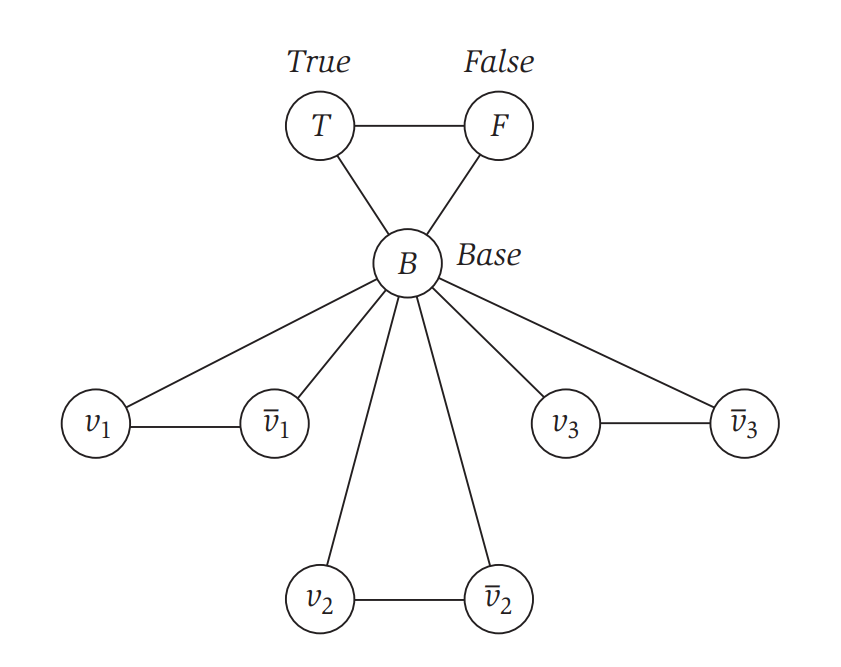
\includegraphics[height=7cm,width=8cm]{figure/1.png}
    \caption{The figure 8.11 from the textbook.}
    \label{1}
\end{figure}

Then, let's build a subgraph for each clause, to ensure that the subgraph is 3-colorable if and only if the clause can be true. The subgraph is showed below for an example $C_i=v_1\lor\bar{v_2}\lor v_3$, and we can easily enumerate the eight cases and find that the subgraph is 3-colorable if and only if at least one of them is true.

\begin{figure}[h]
    \centering
    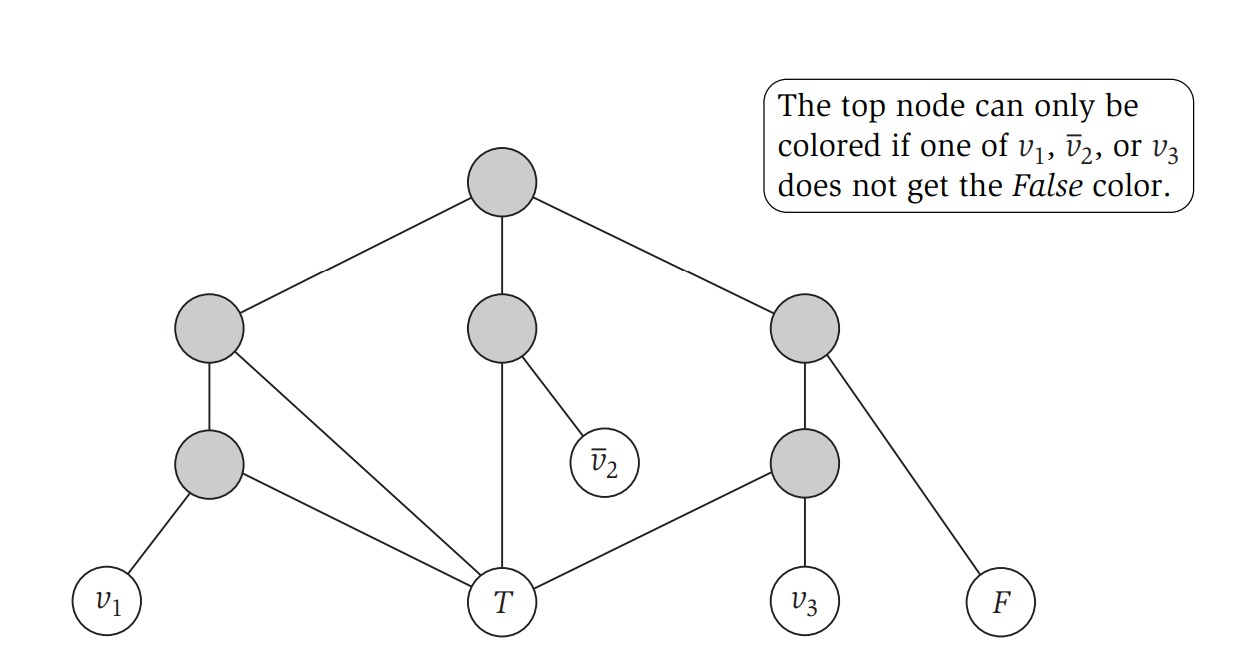
\includegraphics[height=6cm,width=8cm]{figure/2.png}
    \caption{The figure 8.12 from the textbook.}
    \label{2}
\end{figure}

Now, we can build the basic graph and the subgraph for all the clauses, and use the black box to give it a 3-color or tell us that there is no solution. If the black box gives us a solution, then based on our former analysis, each vertex will take the same color with either the true node or the false node, and at least one of each clause will take the same color with the true node, so we can define a satisfying truth assignment based on the coloring. On the contrary, if the black box tells us that there is no solution, then the 3-SAT problem is unsatisfiable, because if it is, then we can also based on the satisfying truth assignment to give the graph a 3-coloring.

Finally, we managed to use a 3-Color problem solver black box and polynomial steps to either solve the 3-SAT problem or prove there is no possible solution, and the black box uses $O(n)$ sized input graph, and only $O(1)$ other steps needed. Therefore, we proved that 3-SAT problem $\leq_p$ 3-Color problem.

\newpage  % reference page

\renewcommand\refname{References}  % change '&' in the link to '\&'
\begin{thebibliography}{99}
    \bibitem[Jon Kleinberg / Éva Tardos(2005)]{textbook} Algorithm Design (Chapter 8)
\end{thebibliography}

\end{document}
